% !TeX spellcheck = id_ID
\documentclass[a4paper,12pt]{article}
\usepackage[indonesian]{babel}
\usepackage{graphicx}
\usepackage{multirow}
\usepackage{enumitem}
\usepackage{listings}
\usepackage{wrapfig}
\usepackage[T1]{fontenc}
\usepackage{inconsolata}
\usepackage{lipsum}
\usepackage{adjustbox}


\usepackage{color}
\usepackage[table]{xcolor}
\definecolor{mygreen}{rgb}{0,0.6,0}
\definecolor{mygray}{rgb}{0.5,0.5,0.5}
\definecolor{mymauve}{rgb}{0.58,0,0.82}
\lstset{%
    language=java,
    showstringspaces=false,          % Prevent tex replacing space to bracket in code
    frame=single,                    % Set frame around code
    backgroundcolor=\color{white},   % choose the background color
    basicstyle=\footnotesize,        % size of fonts used for the code
    breaklines=true,                 % automatic line breaking only at whitespace
    captionpos=b,                    % sets the caption-position to bottom
    commentstyle=\color{mygreen},    % comment style
    escapeinside={\%*}{*)},          % if you want to add LaTeX within your code
    keywordstyle=\color{blue},       % keyword style
    stringstyle=\color{mymauve},     % string literal style
}

\graphicspath{ {./img/} }
\begin{document}
\title{ {\Large Laporan Praktikum}\\ Algoritma dan Pemrograman Lanjut\\{\Large Pertemuan 2}}

\author{Aldzikri Dwijayanto Prathama 
	\\195410189
	\\Informatika}
\makeatletter
\begin{titlepage}
	\begin{center}
		{\huge \bfseries \@title }\\[14ex]
		
\includegraphics[scale=.8]{logo}\\[4ex]
		{\large \@author}\\[12ex]
		{\large \bfseries {SEKOLAH TINGGI MANAJEMEN INFORMATIKA DAN KOMPUTER
				AKAKOM YOGYAKARTA}}
	\end{center}


%{\large \@date} 
\end{titlepage}
\makeatother
%\maketitle
\newpage
\tableofcontents
\newpage

\section{Tujuan}
\paragraph{}
Mahasiswa dapat membuat program untuk menyelesaikan kasus menggunakan
perulangan bertingkat 2 maupun 3

\section{Teori}
\paragraph{}
Dalam Java, ada tiga struktur kontrol perulangan yaitu: for, while, dan do-while.
Untuk yang belum tahu: Perulangan ( atau yang disebut Looping) adalah suatu
proses yang diklakukan secara berulang-ulang hingga mencapai kondisi tertentu.
Sebagai contoh ketika anda ingin mencetak deretan angka hingga batas tertentu
(contoh: 1-100), maka anda bisa menggunakan fungsi looping dalam program.
Biasanya fungsi looping digunakan dan berperan penting dalam algoritma
sorting, karena kita akan menukar nilai variabel hingga menghasilkan nilai
berurutan.

\newpage

\section{Pembahasan}
\subsection{Praktik}
\subsubsection{Praktik 1}
\begin{lstlisting}
public class Looping{
    public static void main(String[] args){
        for (int i=1; i<=2;i++ ) {
            for (int j=1;j<=3 ;j++ ) {
            System.out.format("Perulangan [i=%d, j=%d] %n", i,j);
            }
        }
    }
}
\end{lstlisting}
Perulangan di atas akan mengeprint Perulangan [i=x, j=y] ke layar, di mana x diperoleh dari perulangan yang berada di luar, sedangkan y diperoleh dari perulangan yang ada di dalamnya.\\
Sehingga jika dijalankan, maka akan menghasilkan output berikut:\\
\begin{center}
    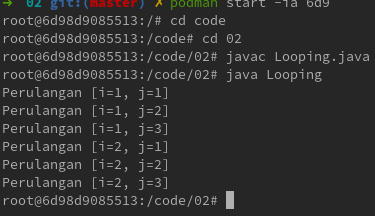
\includegraphics[scale=.7]{1.png}
\end{center}

\begin{lstlisting}
public class Looping{
    public static void main(String[] args){
        for (int i=1; i<=3;i++ ) {
            for (int j=1;j<=2 ;j++ ) {
            System.out.format("Perulangan [i=%d, j=%d] %n", i,j);
            }
        }
    }
}
\end{lstlisting}
Program tersebut sama dengan program sebelumnya, tetapi kondisi pada perulangan diluar dan didalam di tukar, i<=2 menjadi i<=3, sedangkan j<=3 diganti menjadi j<=2.\\
Hasilnya seperti berikut:\\
\begin{center}
    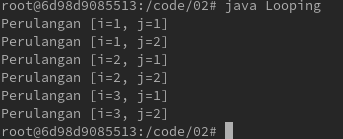
\includegraphics[scale=.7]{2.png}
\end{center}

\subsubsection{Praktik 2}
\begin{lstlisting}
public class Bentuk1
{
    public static void main(String[] args)
    {
        int a = 5;
        for (int b = 1; b <= a; b++)
        {
            System.out.print('*');
            System.out.println();
        }
    }
}
\end{lstlisting}
Program ini memiliki perulangan, yang akan diulang sebanyak 5 kali, yang pernyataannya akan mengeprint bintang, lalu akan mengganti baris. Outputnya seperti berikut:\\
\begin{center}
    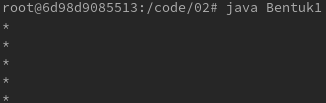
\includegraphics[scale=.7]{3.png}
\end{center}

\newpage

\subsubsection{Praktik 3}
\begin{lstlisting}
public class Bentuk2
{
    public static void main(String[] args) {
        int a = 5;
        for (int b = 1; b <= a; b++){
            for (int c = 1; c <= b; c++) {
                System.out.print('*');
            }
            System.out.println();
        }
    }
}
\end{lstlisting}
Program di atas merupakan program dari praktik 2 yang dimodifikasi dengan menambahkan perulangan di dalam perulangan pertama. Perulangan yang ada didalam akan melakukan perulangan
sejumlah perulangan induknya. Sehinnga program akan menghasilkan output berbentuk segitiga siku-siku seperti berikut:\\
\begin{center}
    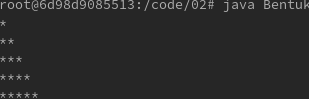
\includegraphics[scale=.7]{4.png}
\end{center}

\subsubsection{Praktik 4}
\begin{lstlisting}
public class Bentuk3
{
    public static void main(String[] args)
    {
        int x = 5;
        for (int i = 1; i <= x; i++)
        {
            for (int j = 4; j >= i; j--)
            {
                System.out.print(' ');
            }
            for (int k = 1; k <= i; k++)
            {
                System.out.print('*');
            }
            for (int l = 1; l <= i - 1; l++)
            {
                System.out.print('*');
            }
            System.out.println();
        }
    }
}
\end{lstlisting}
Program pada praktik 3 dimodifikasi agar bisa menampilkan piramid, sehingga seperti di atas. Perulangan paling luar akan mengulang sebanyak 5 kali, dan 
mempunyai pernyataan yang akan mengganti baris. Lalu di dalamnya terdapat tiga perulangan. Perulangan yang pertama akan mengprint spasi sebanyak 5-i. Perulangan 
kedua akan mengeprint "*" sebanyak i. Sedangkan perulangan terakhir akan mengeprint "*" sebanyak i-1. Jika program dijalankan akan menjadi seperti berikut:\\
\begin{center}
    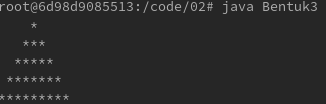
\includegraphics[scale=.7]{5.png}
\end{center}

\subsubsection{Praktik 5}

\begin{lstlisting}
public class Bentuk3a
{
    public static void main(String[] args)
    {
        int x = 5;
        for (int i = 1; i <= x; i++)
        {
            for (int j = 4; j >= i; j--)
            {
                System.out.print(' ');
            }
            for (int k = 1; k <= i; k++)
            {
                System.out.print(k);
            }
            for (int l = 1; l <= i - 1; l++)
            {
                System.out.print(i);
            }
        System.out.println();
        }
    }
}
\end{lstlisting}
Program tersebut merupakan program sebelumnya yang dimodifikasi sehingga akan menampilkan piramid angka. Perulangan paling luar akan mengulang sebanyak 5 kali, dan 
mempunyai pernyataan yang akan mengganti baris. Lalu di dalamnya terdapat tiga perulangan. Perulangan yang pertama akan mengprint spasi sebanyak 5-i. Perulangan 
kedua akan mengeprint variabel k sebanyak i. Sedangkan perulangan terakhir akan mengeprint variabel i sebanyak i-1. Jika program dijalankan akan menjadi seperti berikut:\\
\begin{center}
    
\includegraphics[scale=.7]{6.png}
\end{center}

\subsubsection{Praktik 6}
\paragraph{Program Praktik 2\\}
\begin{center}
\begin{lstlisting}
public class Bentuk1a
{
    public static void main(String[] args)
    {
        int a = 5;
        int b = 1;
        while (b <= a)
        {
            System.out.print('*');
            System.out.println();
            b++;
        }
    }
}
\end{lstlisting}
\end{center}
Program tersebut merupakan program dari praktik 2 yang perulangannya dirubah menjadi while. Sehingga init, dan incrementnya harus dinyatakan sendiri.
Outputnya seperti berikut:\\
\begin{center}
    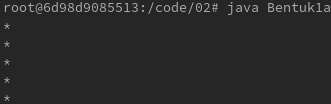
\includegraphics[scale=.7]{7.png}
\end{center}

\paragraph{Program Praktik 5}
\begin{center}
    \begin{lstlisting}
public class Bentuk3a2
{
    public static void main(String[] args)
    {
        int x = 5;
        int i = 1;
        while (i <= x)
        {
            int j = 4;
            while (j >= i)
            {
                System.out.print(' ');
                j--;
            }
            int k = 1;
            while (k <= i)
            {
                System.out.print(k);
                k++;
            }
            int l = 1;
            while (l <= i - 1)
            {
                System.out.print(i);
                l++;
            }
        System.out.println();
        i++;
        }
    }
}
    \end{lstlisting}
\end{center}
Program tersebut merupakan program dari praktik 5 yang perulangannya dirubah menjadi while. Sehingga init, dan incrementnya harus dinyatakan sendiri.
Outputnya seperti berikut:\\
\begin{center}
    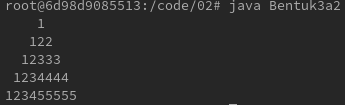
\includegraphics[scale=.7]{8.png}
\end{center}

\paragraph{Program Praktik 3}
\begin{center}
   \begin{lstlisting}
public class Bentuk2a
{
    public static void main(String[] args) {
        int a = 5;
        int b = 1;
        do {
            int c = 1;
            do {
                System.out.print('*');
                c++;
            }while(c <= b);
            System.out.println();
            b++;
        }while(b <= a);
    }
}
   \end{lstlisting} 
\end{center}
Program tersebut merupakan program dari praktik 3 yang perulangannya dirubah menjadi do-while. Sehingga init, dan incrementnya harus dinyatakan sendiri.
Outputnya seperti berikut:\\
\begin{center}
    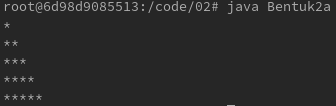
\includegraphics[scale=.7]{9.png}
\end{center}

\paragraph{Program Praktik 4}
\begin{center}
    \begin{lstlisting}
public class Bentuk3b
{
    public static void main(String[] args)
    {
        int x = 5;
        int i = 1;
        do 
        {
            int j = 4;
            do 
            {
                System.out.print(' ');
                j--;
            }while(j >= i);

            int k = 1;
            do 
            {
                System.out.print('*');
                k++;
            }while(k <= i);

            int l = 1;
            do 
            {
                System.out.print('*');
                l++;
            }while(l <= i - 1);

            System.out.println();
            i++;
        }while(i <= x);
    }
}
    \end{lstlisting}
\end{center}
Program tersebut merupakan program dari praktik 4 yang perulangannya dirubah menjadi do-while. Sehingga init, dan incrementnya harus dinyatakan sendiri. Karena perulangan do-while 
akan melakukan perulangan terlebih dahulu, baru melakukan pengecekan, piramid yang dihasilkan tidak rapih.
Outputnya seperti berikut:\\
\begin{center}
    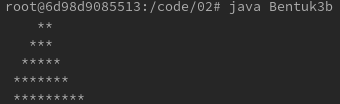
\includegraphics[scale=.7]{10.png}
\end{center}

\newpage

\subsection{Latihan}
\subsubsection{Latihan 1}
\begin{center}
    \begin{lstlisting}
public class Pola1 {
    public static void main(String[] args) {
        int i,j;
        System.out.println("Pengulangan Bersarang Membentuk Pola");
        for(i=1;i<=5;i++){
            for(j=1;j<=3;j++){
                System.out.print(" * ");
            }
            System.out.println("akakom ");
        }
    }
}
    \end{lstlisting}
\end{center}
Program ini memiliki perulangan for, yang di dalamnya terdapat perulangan for lagi. Perulangan yang berada di dalam akan mengeprint bintang sebanyak tiga kali. Lalu perulangan yang paling luar akan mengeprint akakom dan mengganti baris. Outputnya seperti berikut ini:\\
\begin{center}
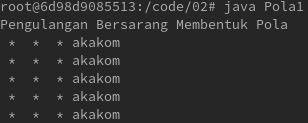
\includegraphics[scale=.7]{11.png}
\end{center}

\newpage

\subsubsection{Latihan 2}
\begin{center}
    \begin{lstlisting}
public class Pola2 {
    public static void main(String[] args) {
        int i,j;
        System.out.println("Pengulangan Membentuk Pola");
        for(i=1;i<=5;i++){
            for(j=1;j<=5;j++){
                if(i>=j){
                    System.out.print(" * ");
                }
            }
            System.out.println("akakom ");
        }
    }
}
    \end{lstlisting}
\end{center}
Setelah program latihan sebelumnya dimodifikasi dengan menambahkan seleksi di dalam perulangan yang berada di dalam, maka program akan menghasilkan segitiga, karena program akan mengeprint "*"
sesuai jumlah baris. Outputnya seperti berikut:\\
\begin{center}
    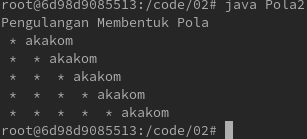
\includegraphics[scale=.7]{12.png}
\end{center}

\subsubsection{Latihan 3}
\begin{center}
    \begin{lstlisting}
public class Pola2a {
    public static void main(String[] args) {
        int i,j,c;
        System.out.println("Pengulangan Membentuk Pola");
        for(i=1;i<=5;i++){
            for(c=1;c<=i;c++){
                System.out.print("   ");
            }
            for(j=5;j>=1;j--){
                if(i<=j){
                    System.out.print(" * ");
                }
            }
            System.out.println("akakom ");
        }
    }
}
    \end{lstlisting}
\end{center}
Agar program menghasilkan segitiga terbalik, ditambahkan perulangan yang akan mengeprint spasi sesuai dengan jumlah baris. Lalu perulangan yang kedua dirubah, yang semula (j=1;j<=5;j++) 
menjadi (j=5;j>=1;j--), dan seleksi yang semula memiliki kondisi i>=j dirubah menjadi i<=j. Maka jika program dijalankan maka akan seperti berikut ini:\\
\begin{center}
    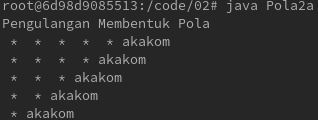
\includegraphics[scale=.7]{13.png}
\end{center}

\newpage

\subsection{Tugas}


\newpage
\section{Kesimpulan}

\end{document}
